\documentclass{article}
\usepackage{graphicx}
\usepackage{multicol}
\usepackage[margin=0.5in]{geometry}
\begin{document}
\title{Matching Trig Graphs B}
\maketitle
\noindent
Write the name of the graph that matches the given equation. Use Graph Sheet
A and your knowledge of graph scaling transformations.
\begin{multicols}{2}
\begin{enumerate}
	\item $y=\sin x$ \hspace{1cm} \rule{5cm}{0.5pt}
	\item $y=-2 \sin x$ \hspace{1cm} \rule{5cm}{0.5pt}
	\item $y=0.5 \cos x$ \hspace{1cm} \rule{5cm}{0.5pt}
	\item $y=1.5 \sin x$ \hspace{1cm} \rule{5cm}{0.5pt}
	\item $y=\sin (2x) $ \hspace{1cm} \rule{5cm}{0.5pt}
	\item $y=\cos(x/3)$ \hspace{1cm} \rule{5cm}{0.5pt}
\end{enumerate}

\noindent
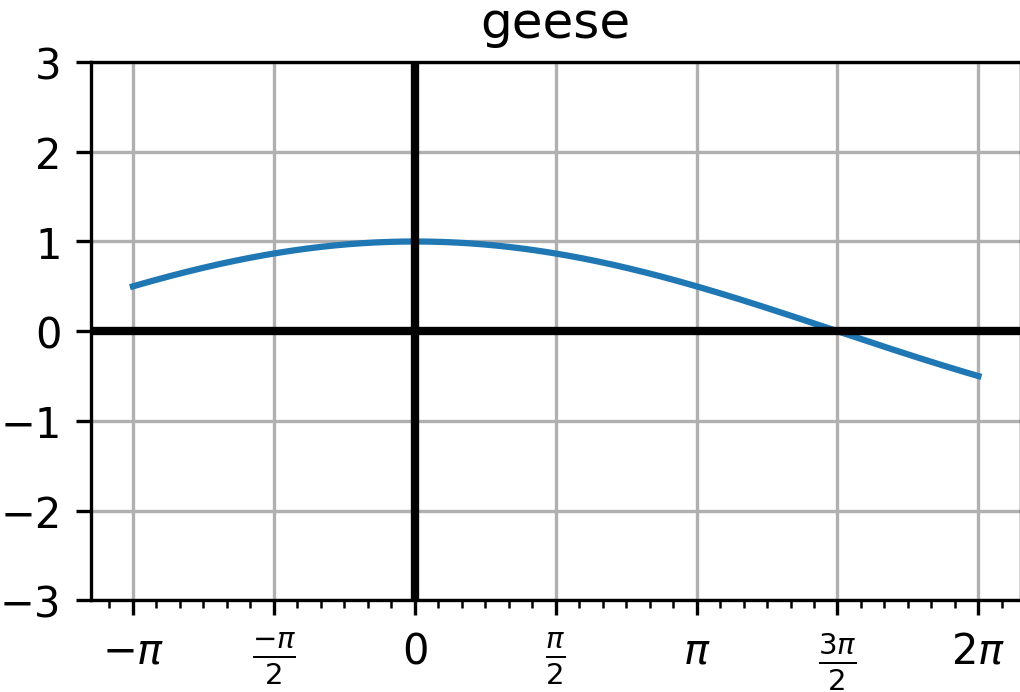
\includegraphics[width=3in]{geese.png} \\
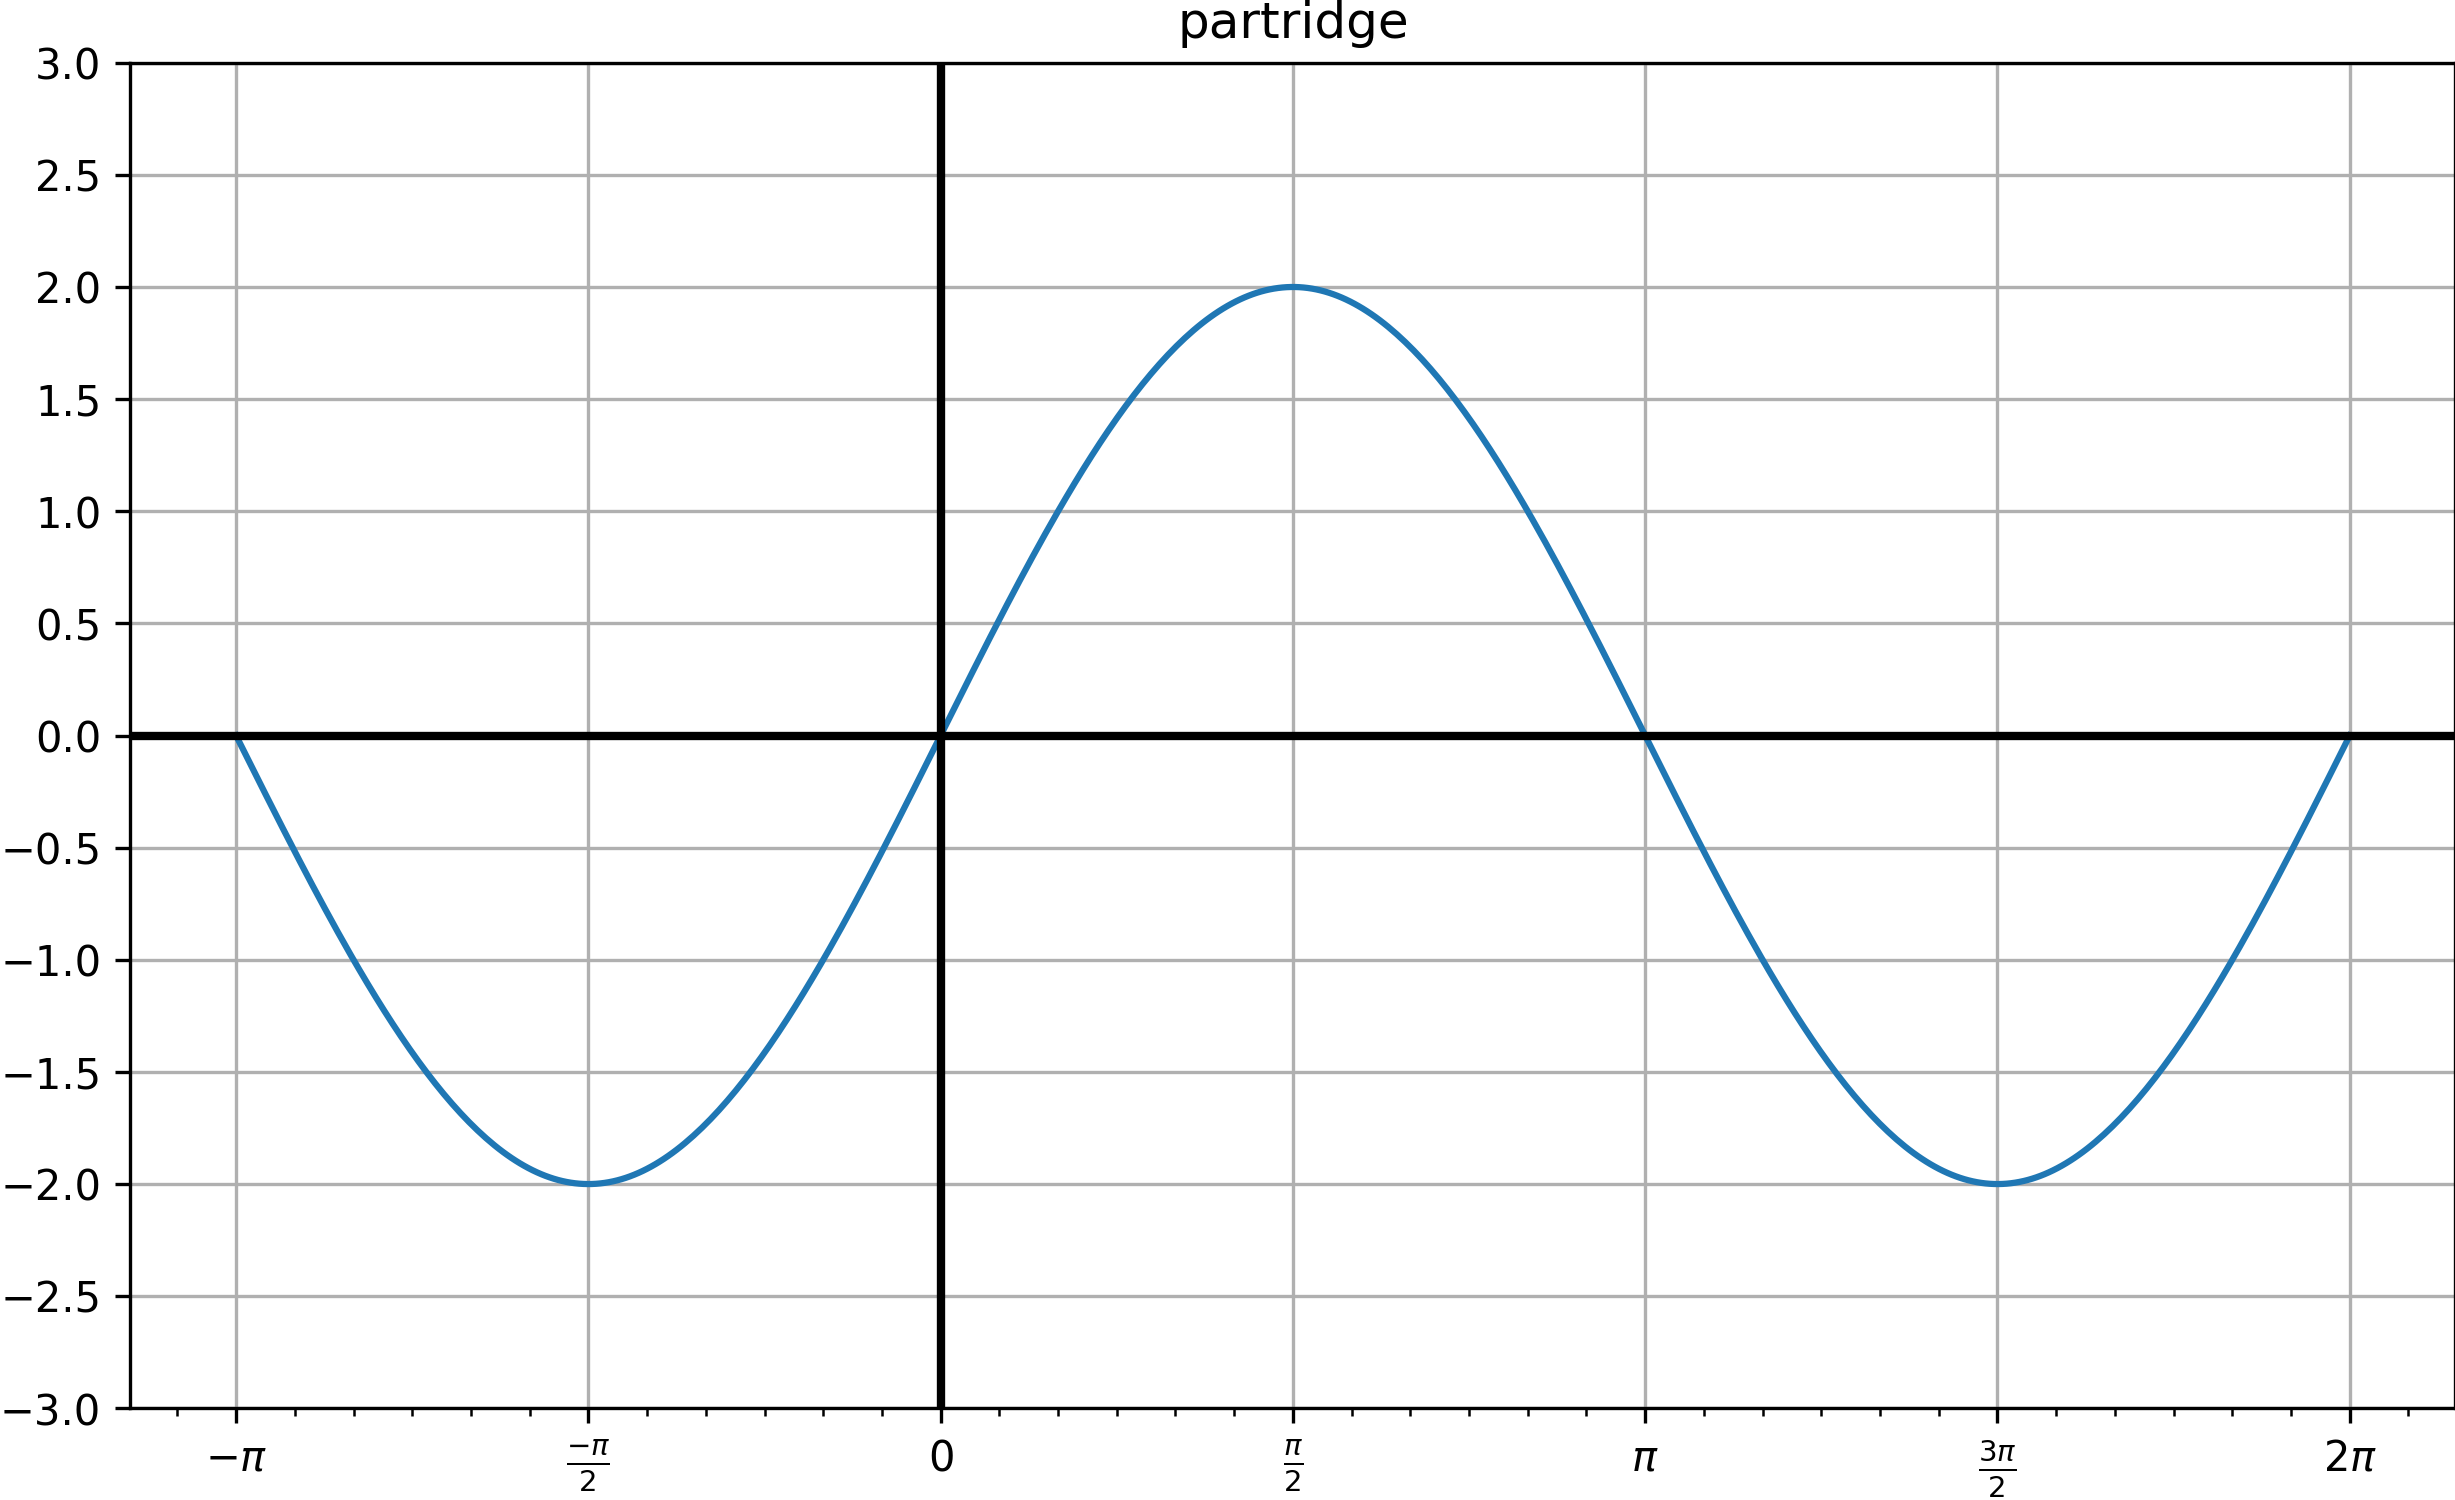
\includegraphics[width=3in]{partridge.png} \\
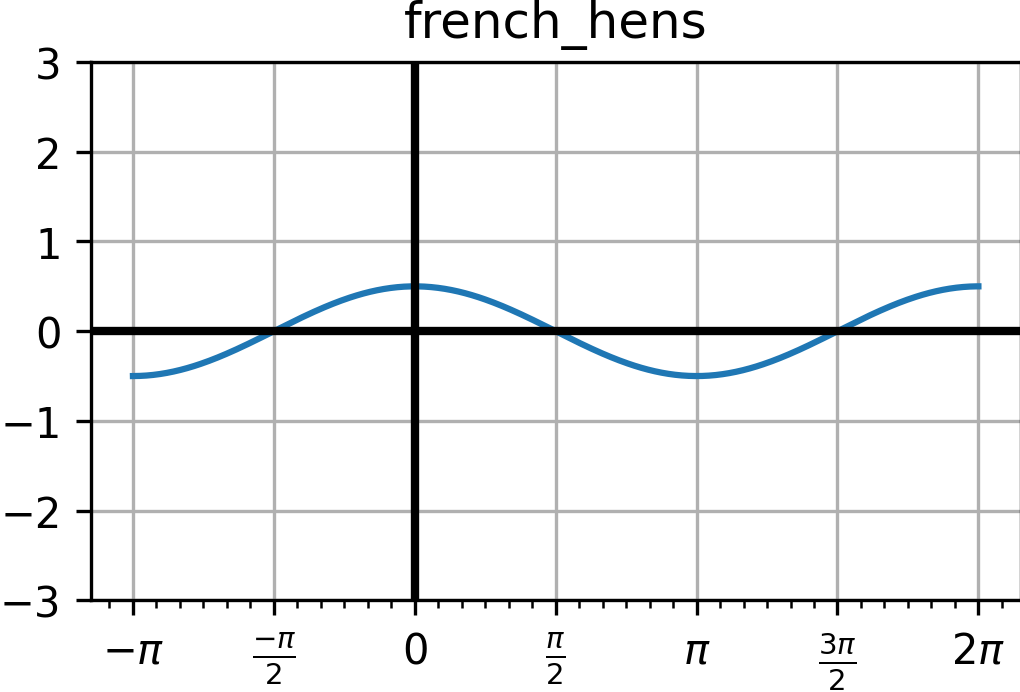
\includegraphics[width=3in]{french_hens.png} \\
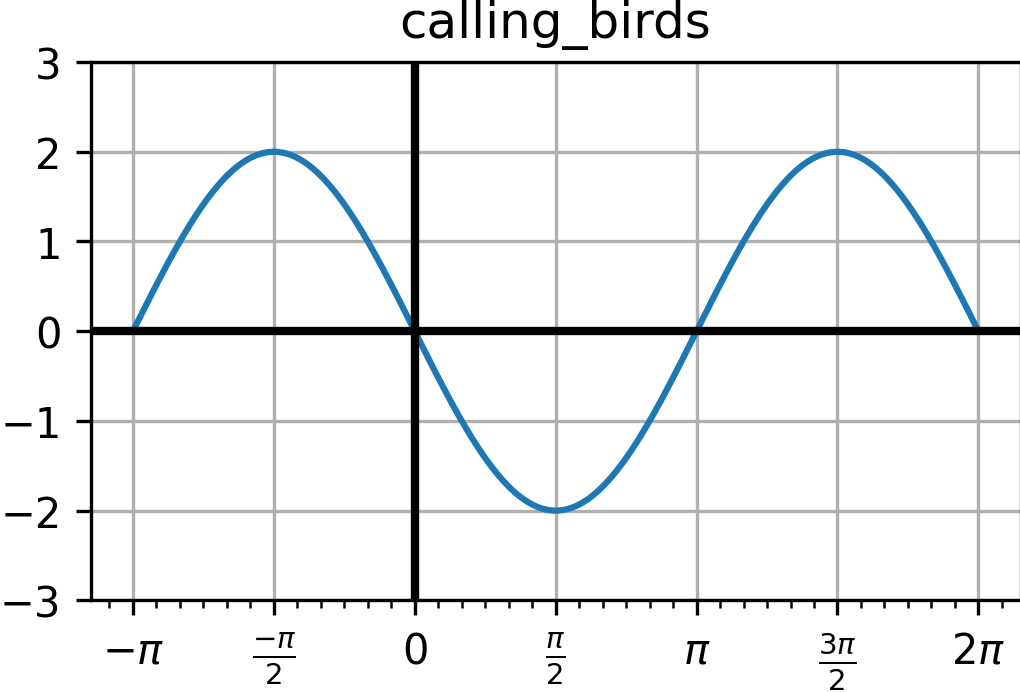
\includegraphics[width=3in]{calling_birds.png} \\
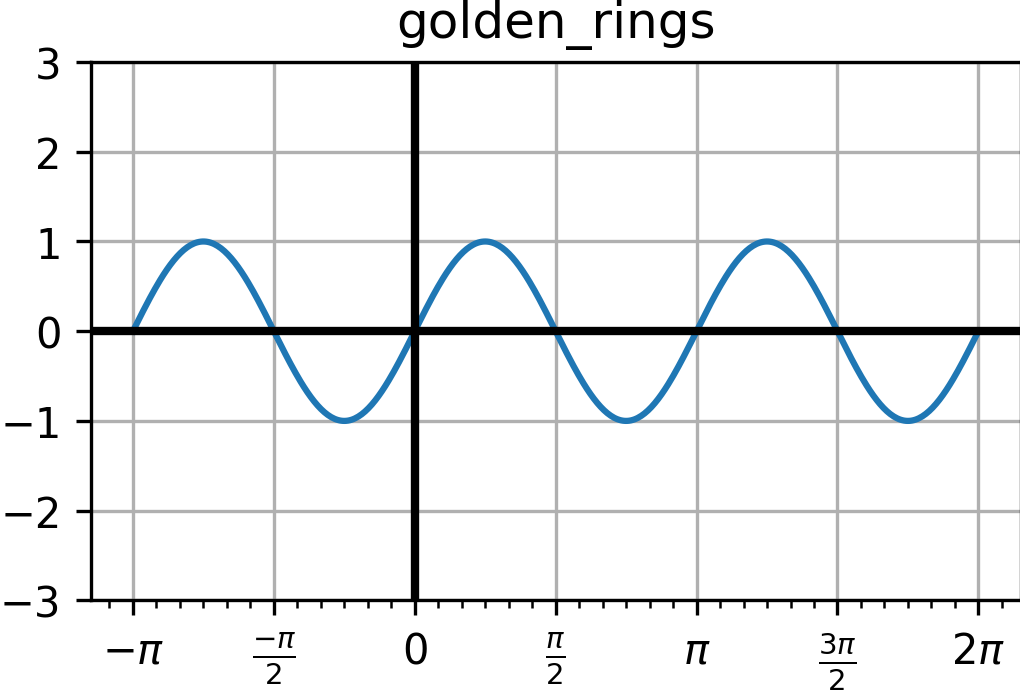
\includegraphics[width=3in]{golden_rings.png} \\
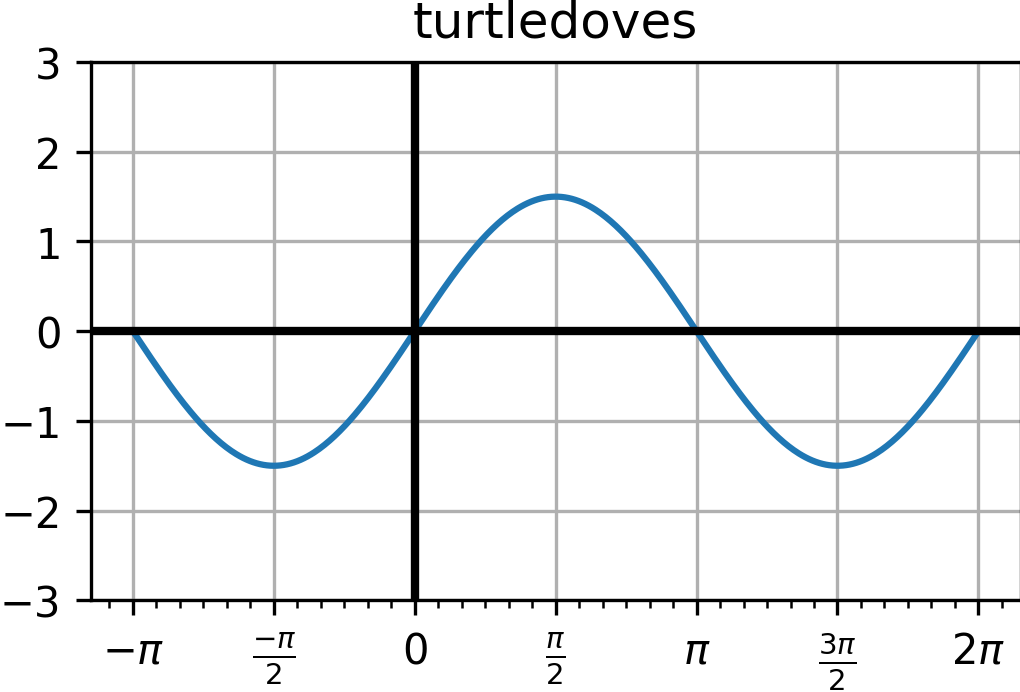
\includegraphics[width=3in]{turtledoves.png}
\end{multicols}
\end{document}
